%% Based on a TeXnicCenter-Template by Gyorgy SZEIDL.
%%%%%%%%%%%%%%%%%%%%%%%%%%%%%%%%%%%%%%%%%%%%%%%%%%%%%%%%%%%%%

%------------------------------------------------------------
%
\documentclass[landscape, notitlepage]{article}%
%Options -- Point size:  10pt (default), 11pt, 12pt
%        -- Paper size:  letterpaper (default), a4paper, a5paper, b5paper
%                        legalpaper, executivepaper
%        -- Orientation  (portrait is the default)
%                        landscape
%        -- Print size:  oneside (default), twoside
%        -- Quality      final(default), draft
%        -- Title page   notitlepage, titlepage(default)
%        -- Columns      onecolumn(default), twocolumn
%        -- Equation numbering (equation numbers on the right is the default)
%                        leqno
%        -- Displayed equations (centered is the default)
%                        fleqn (equations start at the same distance from the right side)
%        -- Open bibliography style (closed is the default)
%                        openbib
% For instance the command
%           \documentclass[a4paper,12pt,leqno]{article}
% ensures that the paper size is a4, the fonts are typeset at the size 12p
% and the equation numbers are on the left side
%
\usepackage{graphicx}
\usepackage{tikz}
\usetikzlibrary{shapes.symbols, 
		shapes.geometric,
		arrows,
		decorations.pathmorphing,
		positioning,
		backgrounds,
		fit}
%-------------------------------------------

\begin{document}
\pagenumbering{gobble}
\topmargin=-10pt
\footskip=0pt
\center\small{SQW Component Interaction: \large{Initial Display upon Login}}

\begin{tikzpicture}[place/.style={
					circle,
					draw=blue!50,fill=blue!20,thick,
					inner sep=0pt,minimum size=6mm},
			component/.style={
					rectangle,
					draw=black!50,fill=blue!20,thick,
					minimum width=3cm,
					inner sep=10pt},
			inlay/.style={
					rectangle,
					draw=black!60,thick,dotted,
					minimum size=15mm,
					inner sep=2pt},
			every label/.style=red,
			end point/.style={circle,fill=red!30,draw=black!30,thick,
						 inner sep=1pt,
						 minimum size=5mm},
			database/.style={cylinder,draw,
						 fill=green!20,
						 aspect=.20,
						 minimum size=1cm,
						 minimum height=1cm+20pt,
						 inner sep=2pt,
						 shape border rotate=90},
			returning/.style={dotted,bend angle=5,bend left},
			this is/.style=dotted,
			bend angle=40,
			pre/.style={<-,shorten <=1pt,>=stealth',semithick},
			post/.style={->,shorten >=1pt,>=stealth',semithick}]
%% -------------- GRID ----------------------------------------- %%
	\path[help lines, blue!20, draw] grid (12,12);

%%  -------------- STICK USER 1 ------------------------------ %%
	\node [xshift=70pt, yshift=-25pt] (user1) at (2, 12)
		{ 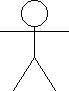
\includegraphics[width=0.6cm]{../img/stick.png}};
	\node [below right=of user1,xshift=-70pt, yshift=15pt] (desktop)
		{ 
\includegraphics[width=0.8cm]{../img/desktop.jpg}}	
		edge[pre, bend left] (user1);
		
%%  -------------- STICK USER 2 ------------------------------ %%
	\node [right=of user1, xshift=2cm, yshift=-6pt] (user2)
		{ 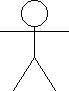
\includegraphics[width=0.6cm]{../img/stick.png}}; 
	\node [below right=of user2, xshift=-25pt, yshift=20pt] (mobile)
				{ 
\includegraphics[width=0.8cm]{../img/mobile.jpg}}
		edge[pre, bend right] (user2);	 
	\node [xshift=3pt, yshift=4pt,right=of user1] {Users}
		edge[this is] (user1)
		edge[this is] (user2);


%% -------------- WEB SITE COMPONENT --------------------- %%
	\node [ component,below left=of desktop, xshift=1.3cm,yshift=15pt] (web)
									 {Web Site}
		edge[pre, bend left] (desktop);

%% ------------------------------ GATEWAY----------------------- %%
	\node [ component,below right=of web, 
			minimum height=1.5cm,
 			xshift=-3.5cm,yshift=5pt] (gateway) {Gateway};

	%% phantom node for return arrow from KV store
	\node [right=of gateway, xshift=-1.25cm, yshift=-2pt] (gateway_kvback) {};

%% -------------------------------- CONNECTIONS ----------------- %%
	\node[end point, above=of gateway, xshift=0.3cm,yshift=-1.55cm] 
							(conn1)	{}
		edge[pre] (web);
	\node[end point, right=of conn1, xshift=-.8cm,yshift=-2pt] 
							(conn2)	{}
		edge[pre] (mobile);

%% --------------------------------- KV Store ---------------------- %%
	\node[database, right=of gateway, xshift=1.7cm] (kvstore) {K-V Store}
		edge[pre] (gateway)
		edge[post,returning] (gateway_kvback);

%% ---------------------------------- SERVICE ---------------------- %%
	\node[component, below=of gateway, 
			minimum width=4cm, xshift=5pt, yshift=-10pt,
			text depth=2cm] (service) {Service}
		edge[pre] (gateway);	
	\node[inlay, above=of service,
		  yshift=-3.8cm,xshift=-1cm-5pt] (cache) {cache};

%% ----------------------------------- DATASYS ---------------------- %%
	\node[component, right=of service, fill=black!20,
			minimum height=2cm,
			xshift=2cm+15pt,yshift=-25pt] {Data System}
		edge[pre,dotted] (service);

%% ------------------------------------ BACGROUND ----------------- %%
	\begin{pgfonlayer}{background}
		\node [fill=red!10,align=left,
				fit=(gateway) (gateway_kvback) (kvstore) (service)]
			{SqrWall Core};
	\end{pgfonlayer}
\end{tikzpicture}


\end{document}
